% !TEX encoding = UTF-8 Unicode
% !TEX root = thesis-ex.tex
This chapter shall discuss some important experimental jet measurements that motivate the study of the main analysis in this thesis. It will begin with a brief discussion of the jet reconstruction procedure and go on to discuss measurements of jet yields, dijet asymmetry, and jet fragmentation. 

%These measurements include the jet $\mathrm{R}_{AA}$, jet $\mathrm{X}_{J}$, and jet fragmentation. 
\section{Jet Reconstruction}
Jets can reconstructed by clustering algorithms that take in a variety of inputs. The algorithm used in ATLAS is the \antikt\ clustering algorithm \cite{Cacciari:2008gp}. This algorithm clusters soft particles around hard ones in the following manner:

\begin{itemize}
\item Calculate all distances $d_{ij}$ between entities $i$ and $j$, and distance $d_{iB}$ between entity $i$ and beam $B$.
\item Identify the smallest distances such that for the smallest distance $d_{ij}$, the entities $i$ and $j$ are combined and return to beginning.
\item If the smallest distance is $d_{iB}$, then take $i$ as the jet and remove it from the list of entities and return to beginning.
\item Continue the procedure till the list of items is empty.
\end{itemize}

In general the distance $d_{ij}$ between the objects is found the via the prescription

\begin{align}
d_{ij} &= \mathrm{min} (k_{Ti}^{2p} , k_{Tj}^{2p}) \frac{\Delta_{ij}^2}{R^2}  \\
d_{iB} &= k_{Ti}^{2p}
\end{align}

where $k_{Ti}$ is the transverse momentum of particle $i$ and $\Delta_{ij} = \sqrt{\Delta\eta_{ij}^2 + \Delta\phi_{ij}^2}$ is the distance between particles $i$ and $j$ in $\eta-\phi$ space. $R$ the distance parameter and reflects the size of the jet being considered. In the case of the \antikt\ algorithm, $p = -1$. Other popular clustering algorithms like \kt\ \cite{Catani:1993hr} and Cambridge/Aachen \cite{Dokshitzer:1997in} use $p = 1$ and $p=0$ respectively. The behavior of the different clustering algorithms is shown in Figure~\ref{fig:JetClustering}. 

\begin{figure}[htp]
\centering
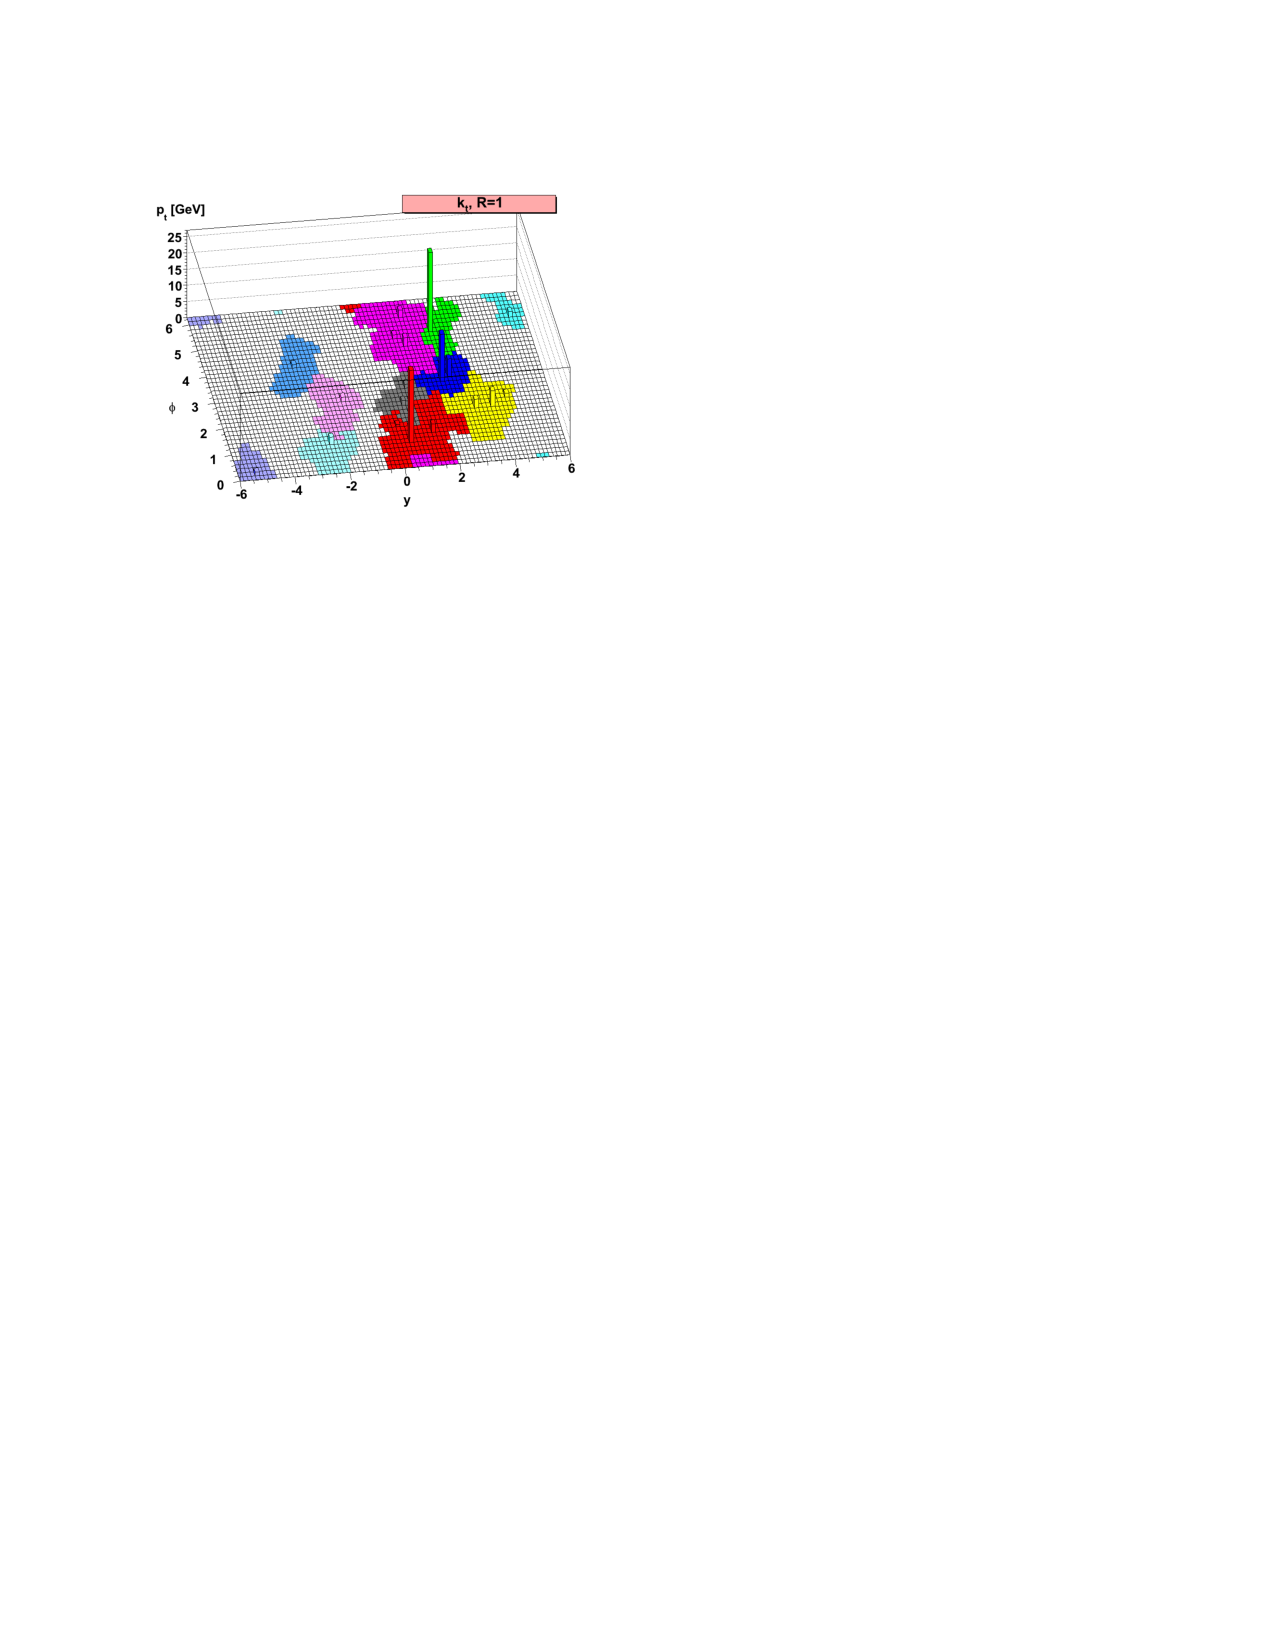
\includegraphics[width=.3\textwidth]{jetMeasurements/jetReco_kt}\hfill
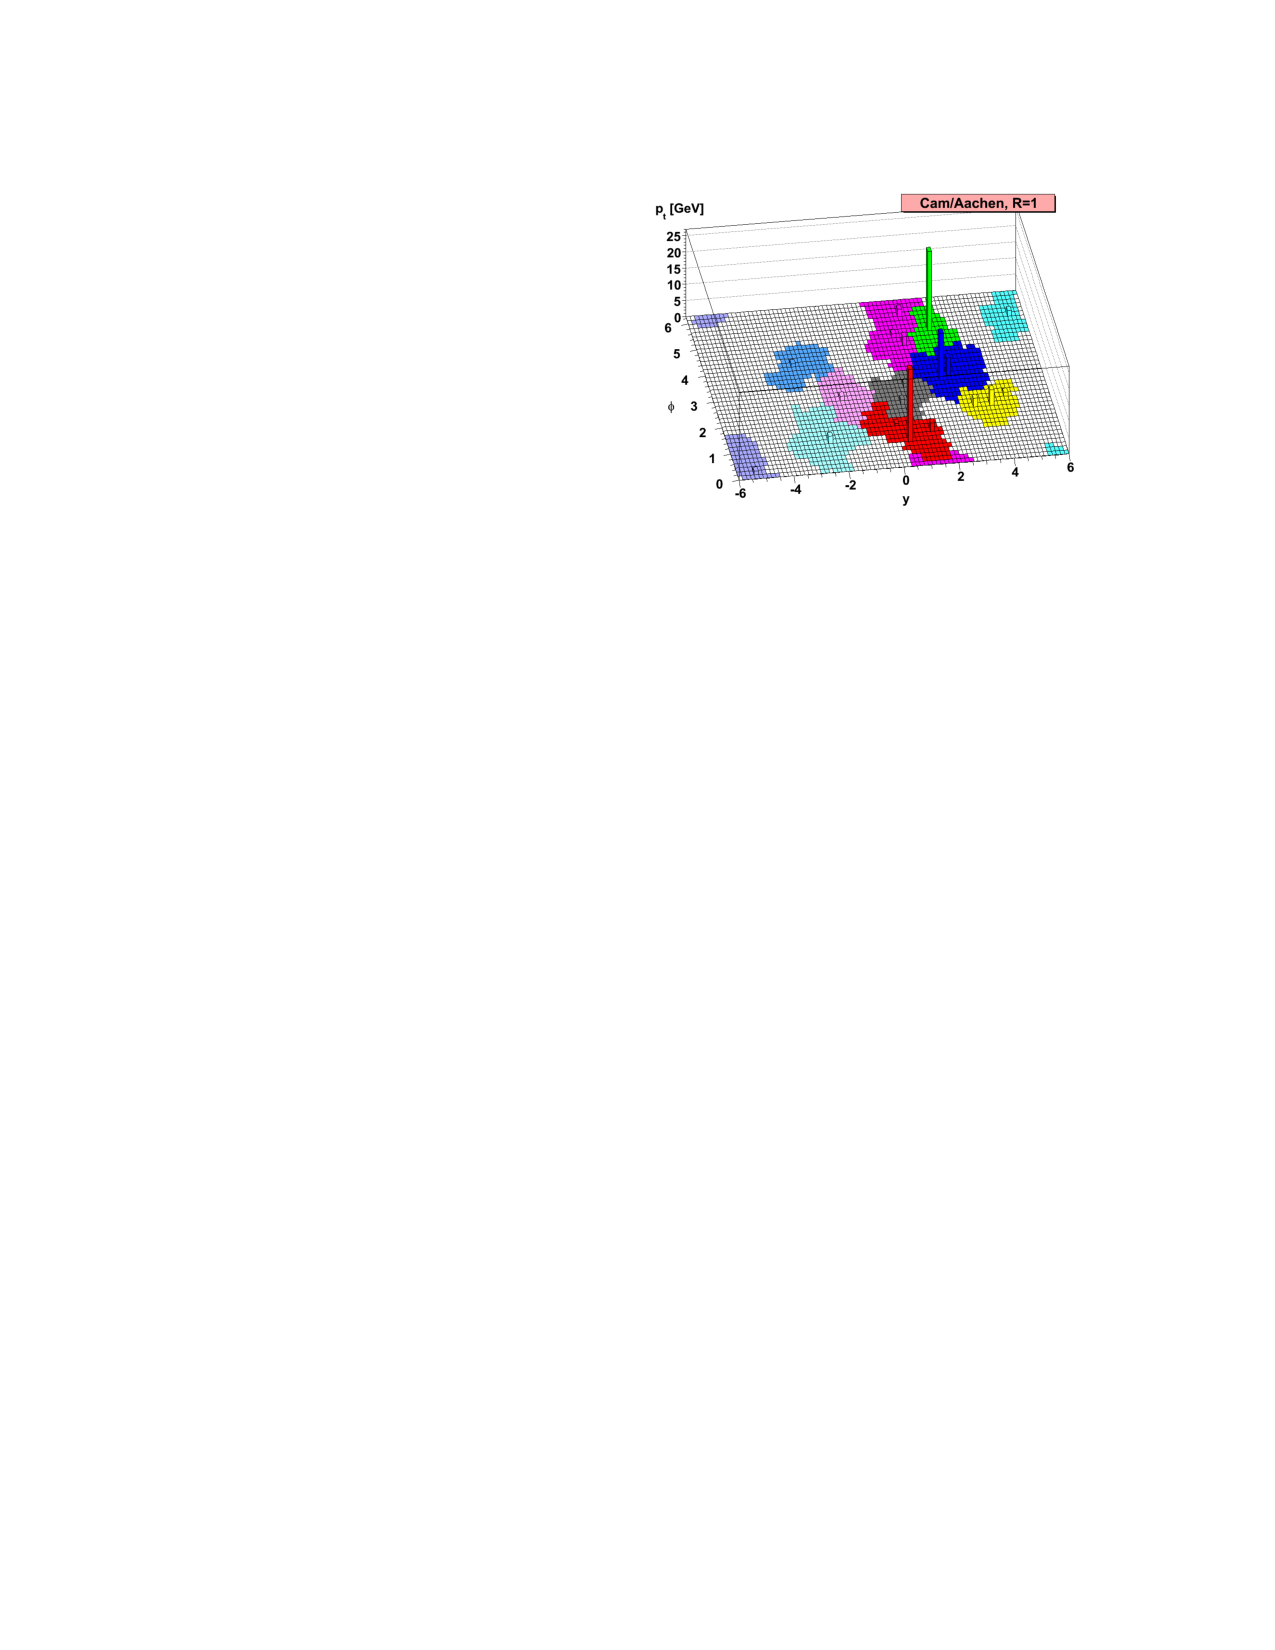
\includegraphics[width=.3\textwidth]{jetMeasurements/jetReco_CA}\hfill
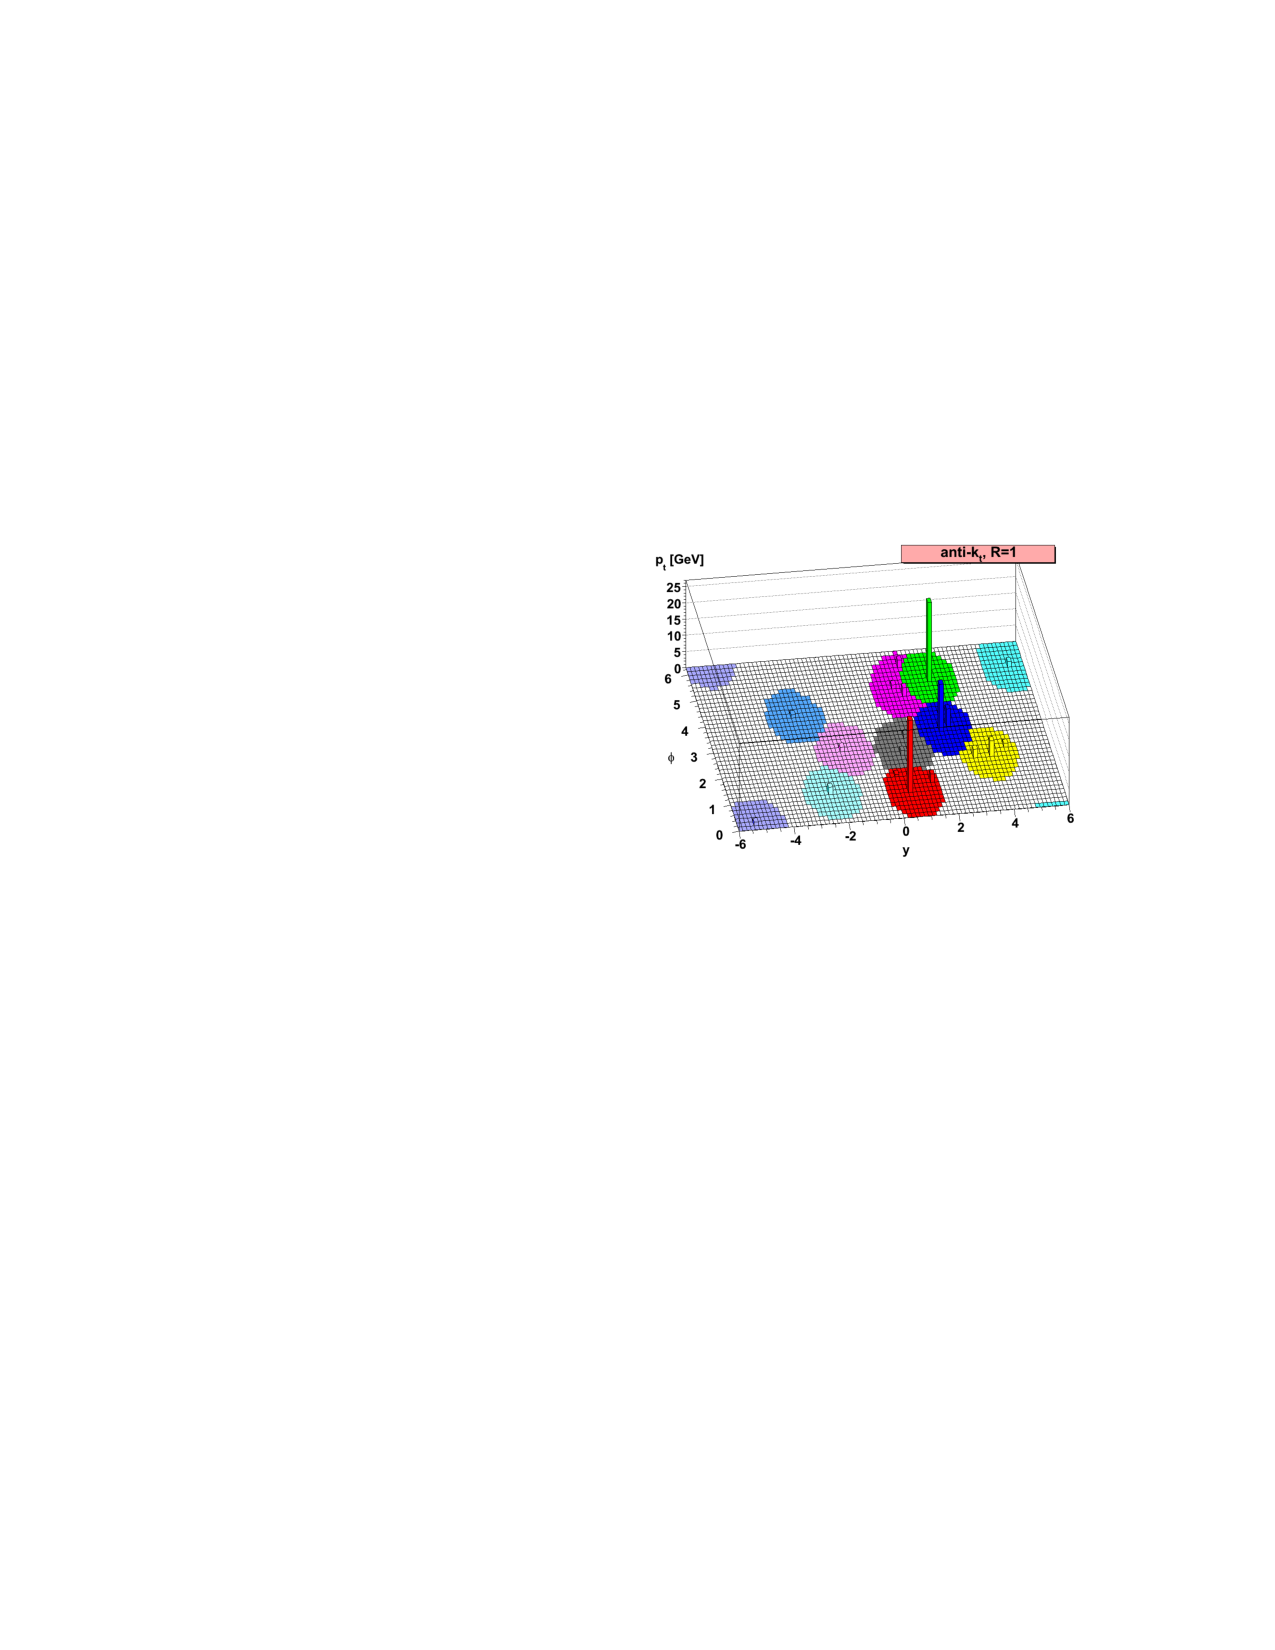
\includegraphics[width=.3\textwidth]{jetMeasurements/jetReco_antikt}\hfill
\caption{Different clustering algorithms applied to the sample parton-level event. Figure taken from \cite{Cacciari:2008gp}.}
\label{fig:JetClustering}
\end{figure}

The popularity of the \antikt\ algorithm comes from its overcoming of two common problems: collinear and infrared safety. These are related to instabilities in the cones that are found due to soft radiation. 

Figure~\ref{fig:collinearSafe} describes the collinear safety problem. In a collinear safe jet algorithm, the presence of a virtual loop or a collinear splitting of a central particle would not change the number of jets being reconstructed. On the other hand, while a collinear unsafe jet algorithm would not change its output with the presence of a virtual loop, a splitting in the central particle would lead to the left and right most particles forming individual seeds, implying two reconstructed jets \cite{Salam:2009jx}.

\begin{figure}[htp]
\centering
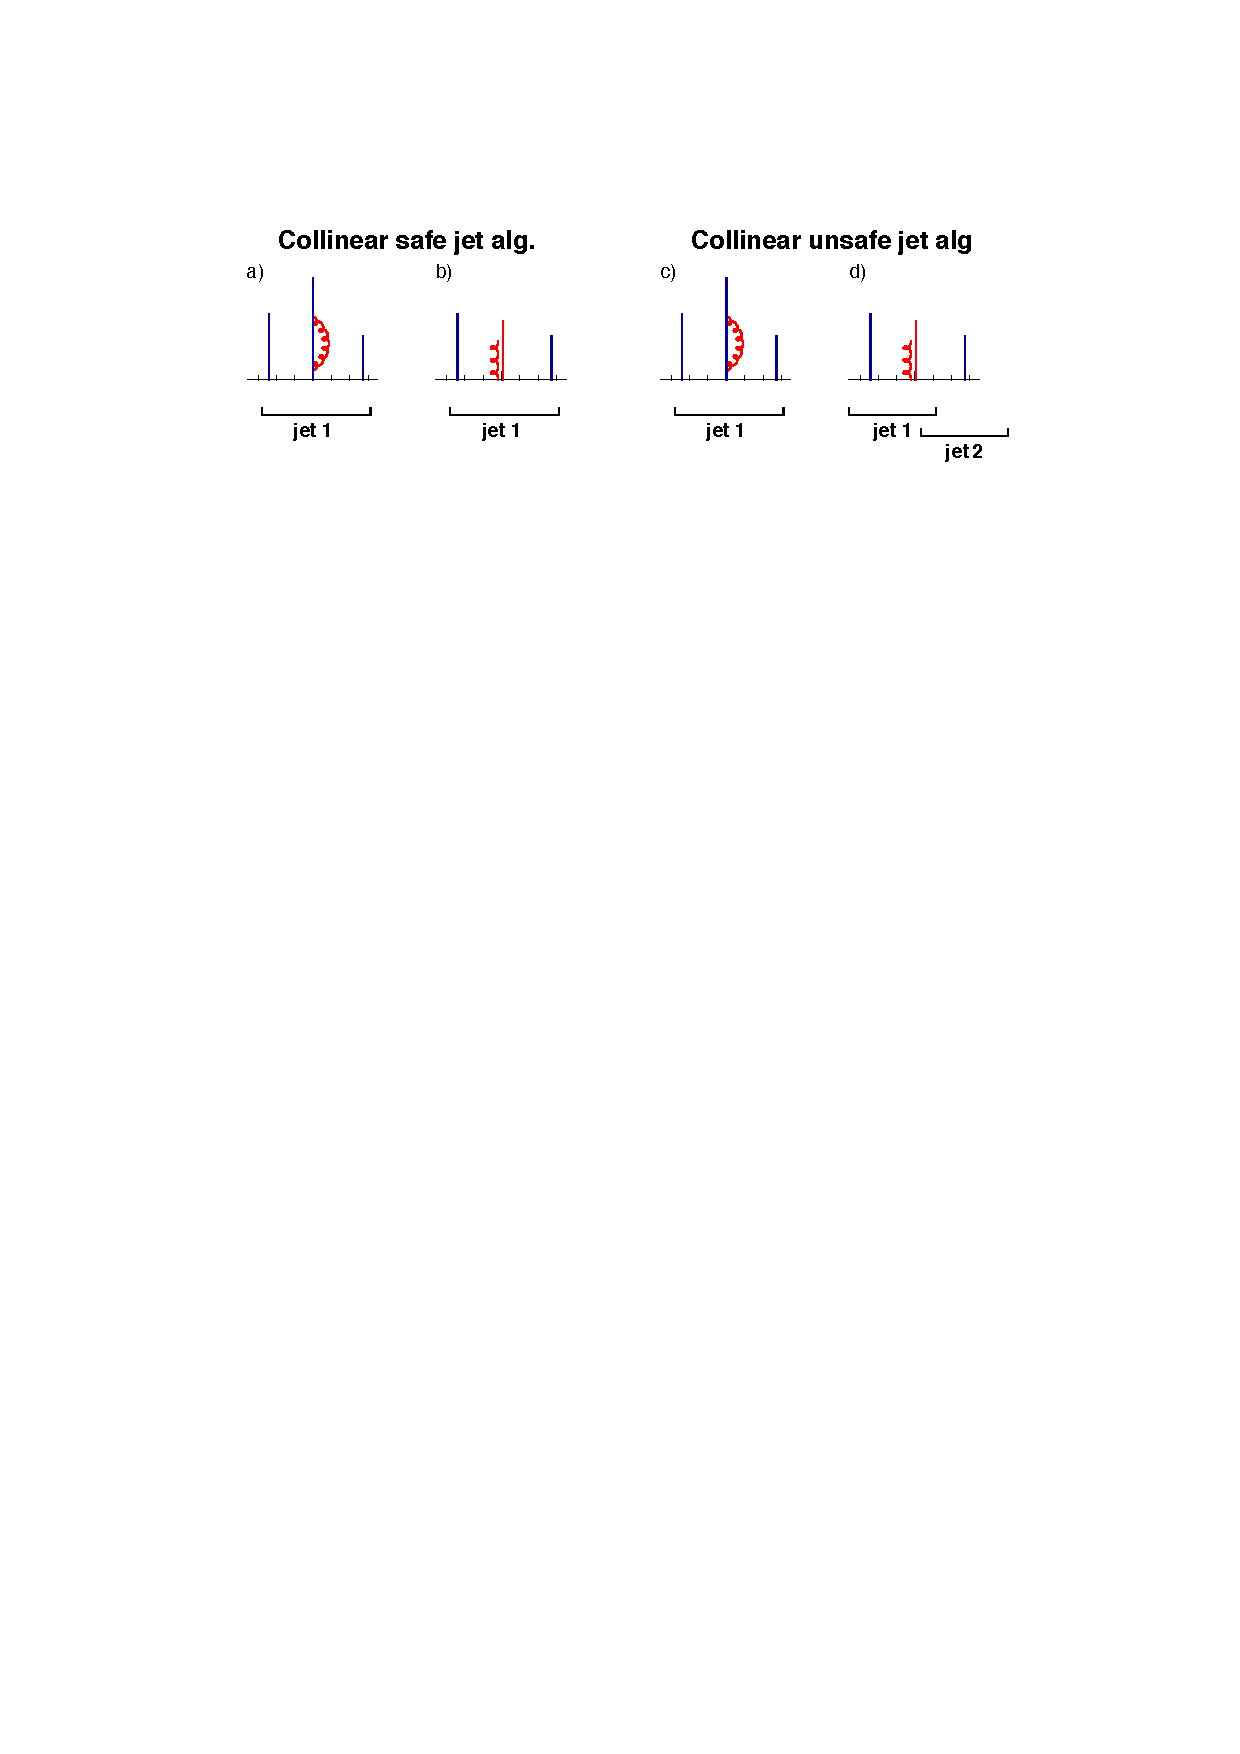
\includegraphics[width=.75\textwidth]{jetMeasurements/collinearSafe}
\caption{An illustration of collinear unsafe behavior. The particle \pt\ is proportional to the height and the horizontal axis indicates rapidity. Taken from \cite{Salam:2009jx}. }
\label{fig:collinearSafe}
\end{figure}


A schematic describing infrared un-safety is shown in Figure~\ref{fig:infraredSafe}. Here an infrared safe algorithm would use the three particles as seeds iteratively find two stable cones. An unsafe algorithm however would find three overlapping cones based on the addition of a soft seed.

\begin{figure}[htp]
\centering
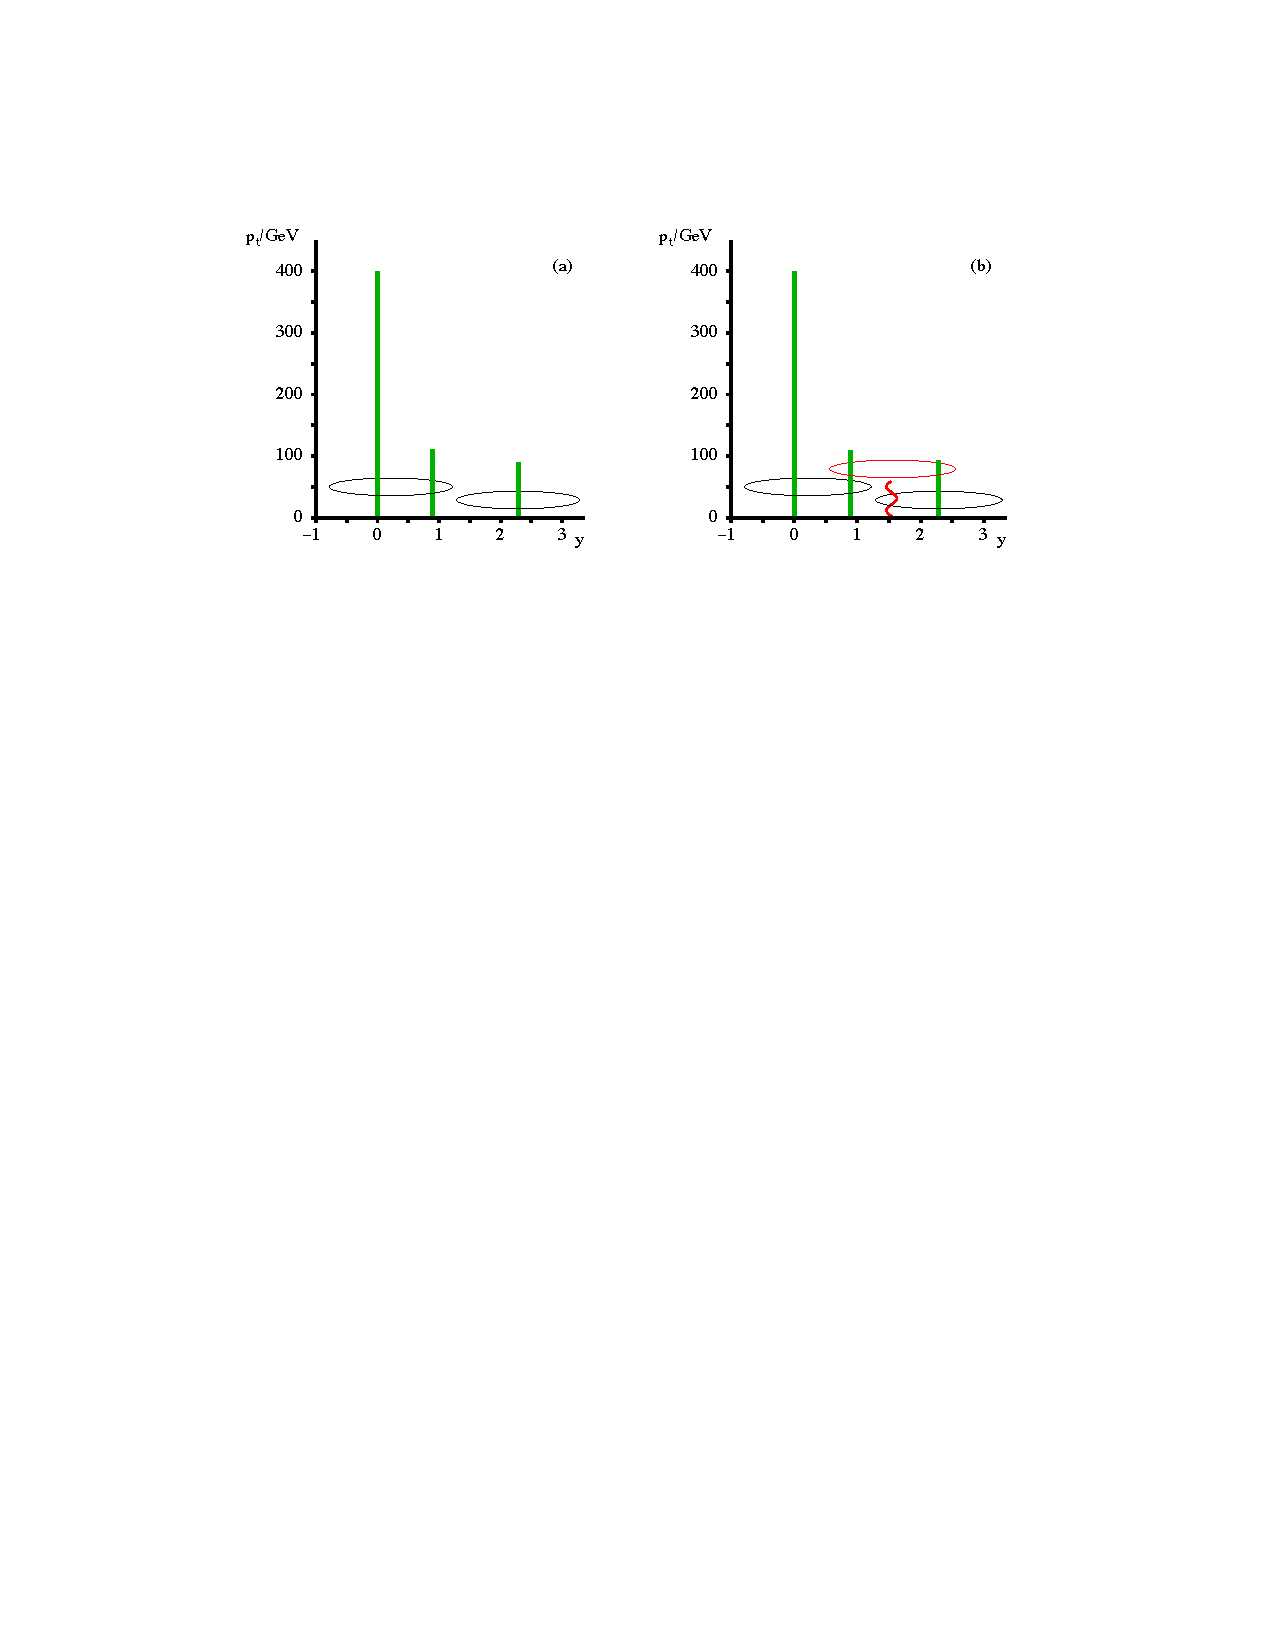
\includegraphics[width=.65\textwidth]{jetMeasurements/infraredSafe}
\caption{An illustration of infrared unsafe behavior. The particle \pt\ is proportional to the height and the horizontal axis indicates rapidity. Taken from \cite{Salam_2007} }
\label{fig:infraredSafe}
\end{figure}

% the \antikt\ reconstruction algorithm is used with the distance parameter $R=0.4$

For heavy ion collisions in ATLAS, the inputs to the algorithm are the $\eta \times \phi = 0.1 \times 0.1$ calorimeter towers. The tower energies are determined by summing up the energies of the individual calorimeter cells. The \antikt\ algorithm is first run with the distance parameter $R=0.2$, following which an underlying event subtraction procedure is performed. A first estimate of the average underlying event energy density $\rho_i (\eta)$ is done in 0.1 slices of $\eta$ in each calorimeter layer $i$ after excluding the regions that overlap with the seed jets. A modulation of $2v_{2} \cos[2(\phi-\Psi_2)] $ is applied to account for the flow from the QGP and the underlying event is subtracted to give $E_{Tj}^{\mathrm{sub}}$:

\begin{align}
E_{Tj}^{\mathrm{sub}} = E_{Tj} - A_j \rho_i (\eta_j) 1+2v_{2i} \big(\cos[2(\phi-\Psi_2)] \big)
\end{align}
where $ E_{Tj} , \eta_j, \phi_j$ and $A_j$ are the cell $E_T, \eta, \phi$ and area for cell $j$ in layer $i$. This process is done iteratively done one more time after getting new seeds with the distance parameter $R = 0.2$ and excluding areas that are within $\Delta R = 0.4$ of the seeds. Updated values of $\rho{'}_i$ and $v{'}_2$ are recalculated and used to estimate the background that is subtracted from the original cell energies. More details on this procedure can be found in \cite{2013220}

























\section{Modification of jet yields: {\textsc Jet $\mathrm{R}_{AA}$} }
{\textsc Jet $\mathrm{R}_{AA}$} and {Jet $\mathrm{R}_{AA}$}

%Experimentally, the nuclear modification can be quantified by the nuclear modification factor $R_{AA}$:
%
%\begin{align}
%R_{AA} (\pt, y, \phi_p) = \frac{1}{N_{\mathrm{coll}}}
%\end{align}





\section{Jet $\mathrm{X}_{J}$}
\section{Jet Fragmentation}



